\listoftodos


\chapter{Werkzeuge}
\label{chap:Werkzeuge}

	\section{SecondCriterionAutoenocder}
	\label{sec:SecondCriterionAutoenocder}
		
		
		
		\begin{figure}[h]
			\centering
			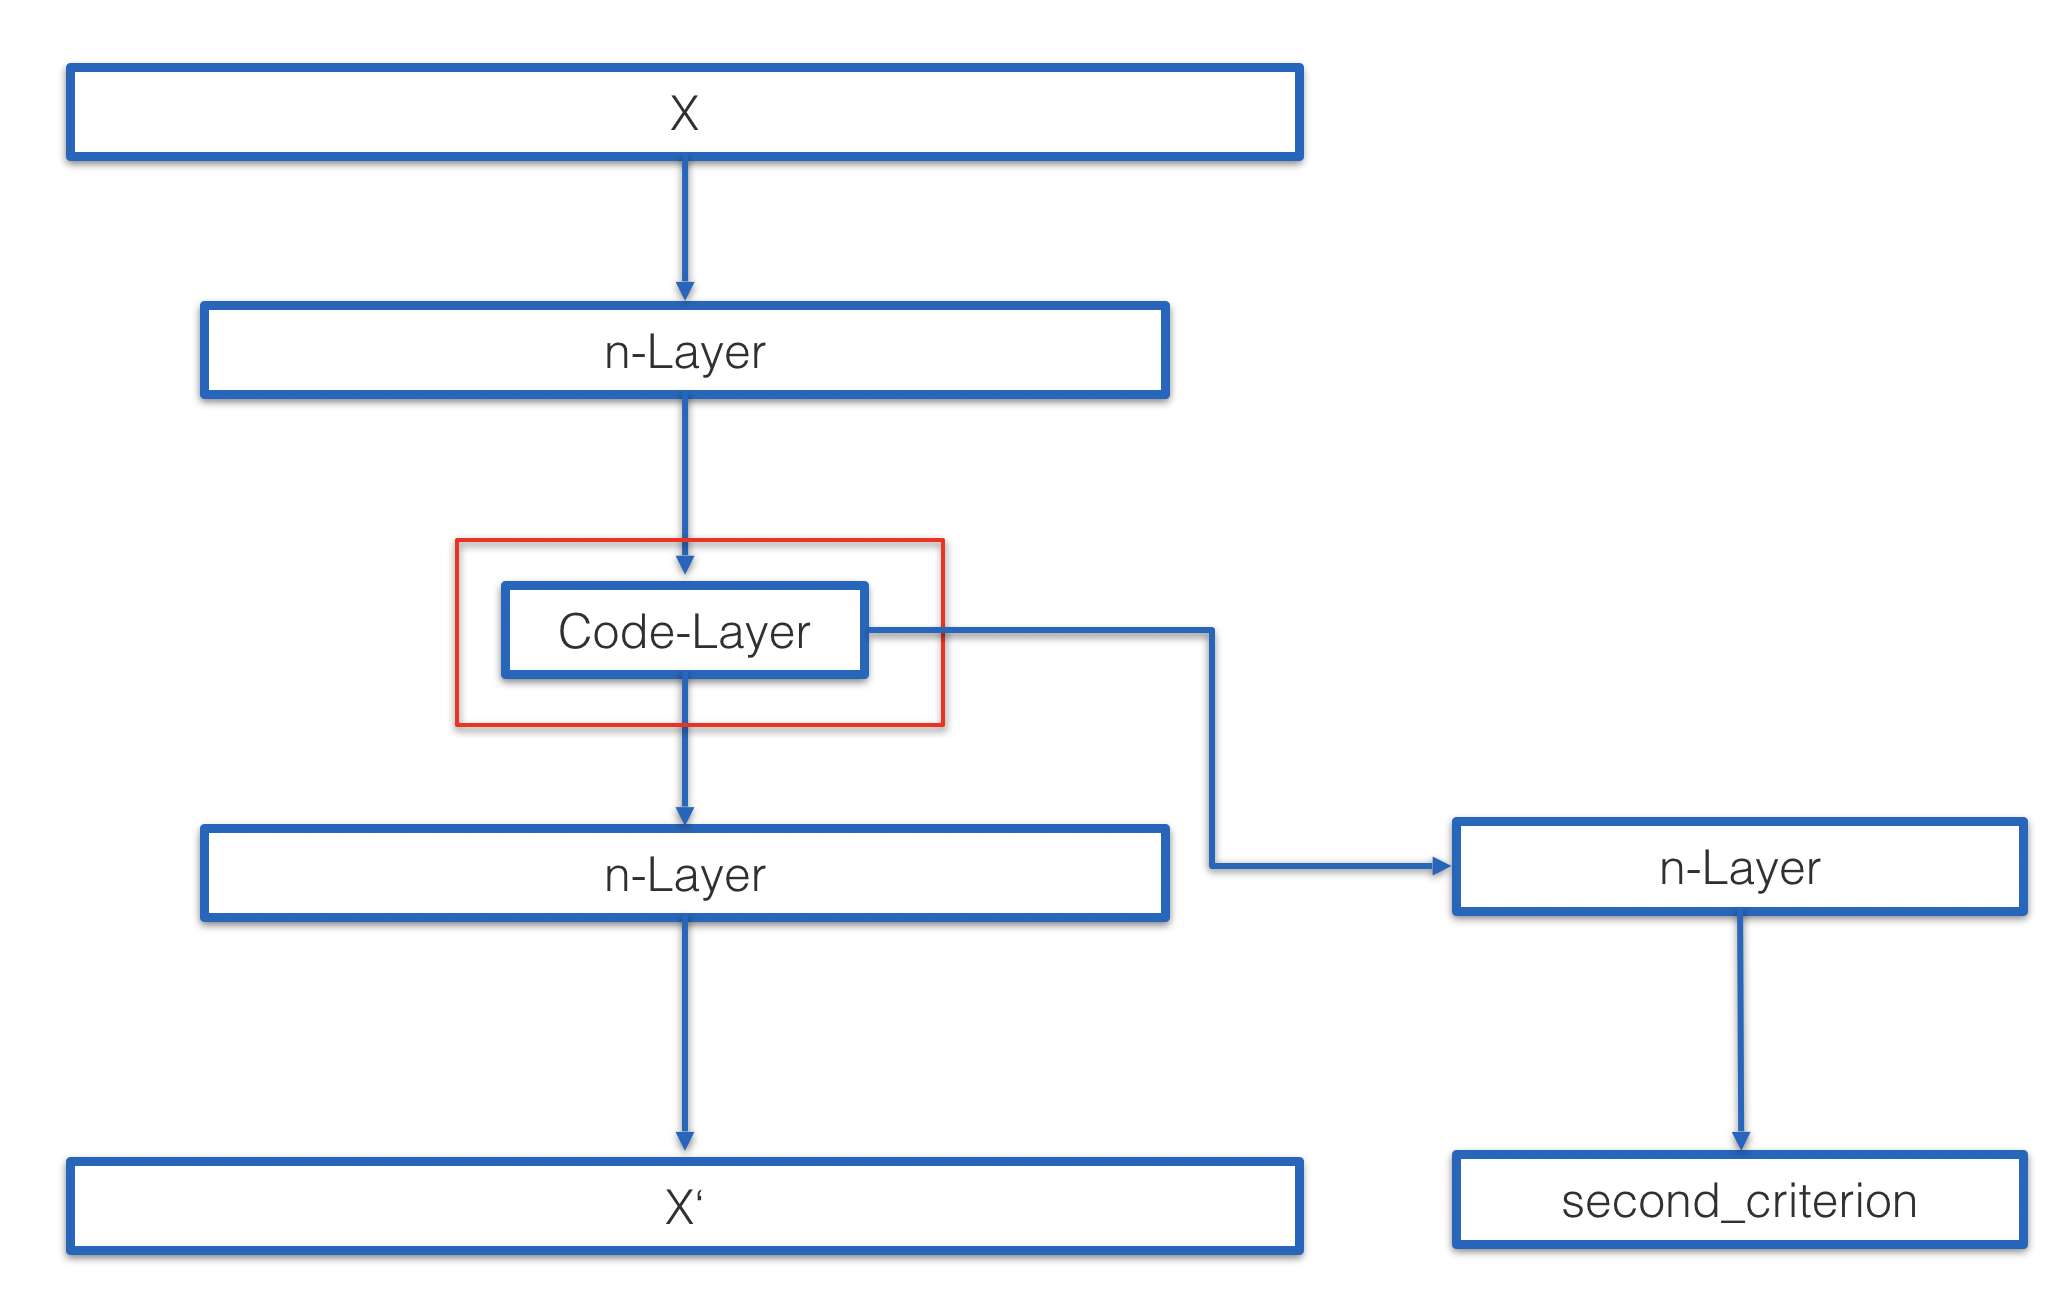
\includegraphics[width=0.5\textwidth, center]{bilder/Schema_Autoencoders/Schema_SCAE.png}
			\caption[Schema SecondCriterionAutoenocder]{Schema SecondCriterionAutoenocder}
			\label{img:SchemaSCAE}
		\end{figure}  
		
		
		\begin{figure}[h]
			\centering
			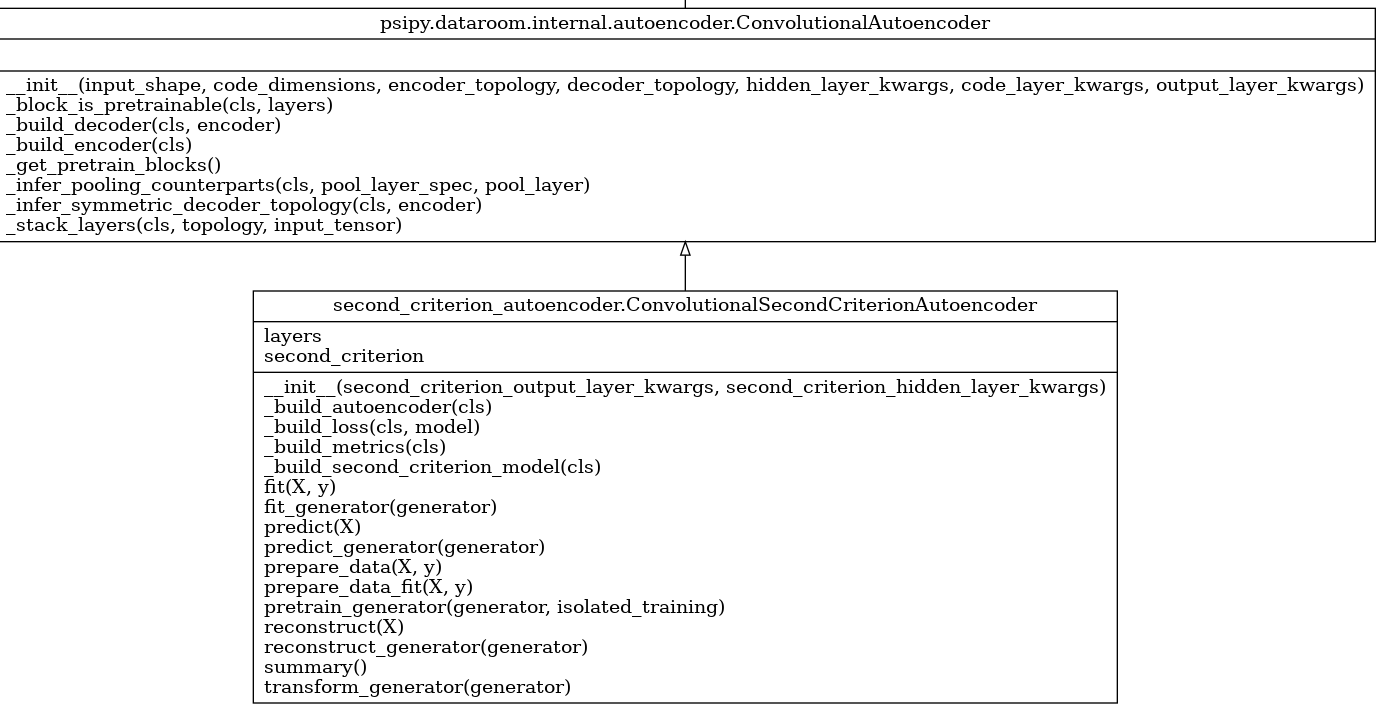
\includegraphics[width=0.5\textwidth, center]{bilder/Klassendiagramme/Klassendiagramm_CSCAE.png}
			\caption[Klassendiagramm ConvolutionalSecondCriterionAutoencoder]{Klassendiagramm ConvolutionalSecondCriterionAutoencoder}
			\label{img:KlassendiagrammCSCAE}
		\end{figure}  
		
		Warum pretrian?:	https://papers.nips.cc/paper/3048-greedy-layer-wise-training-of-deep-networks.pdf (Warum machen das andere heute nicht mehr? viele cnn haben vanishing gradients problem  über relu,... gelösst) (weitere literatur: möglicherweise Geoffrey E. Hinton)

	\section{TransferSecondCriterionAutoenocder}
	\label{sec:TransferSecondCriterionAutoenocder}

	\begin{figure}[h]
		\centering
		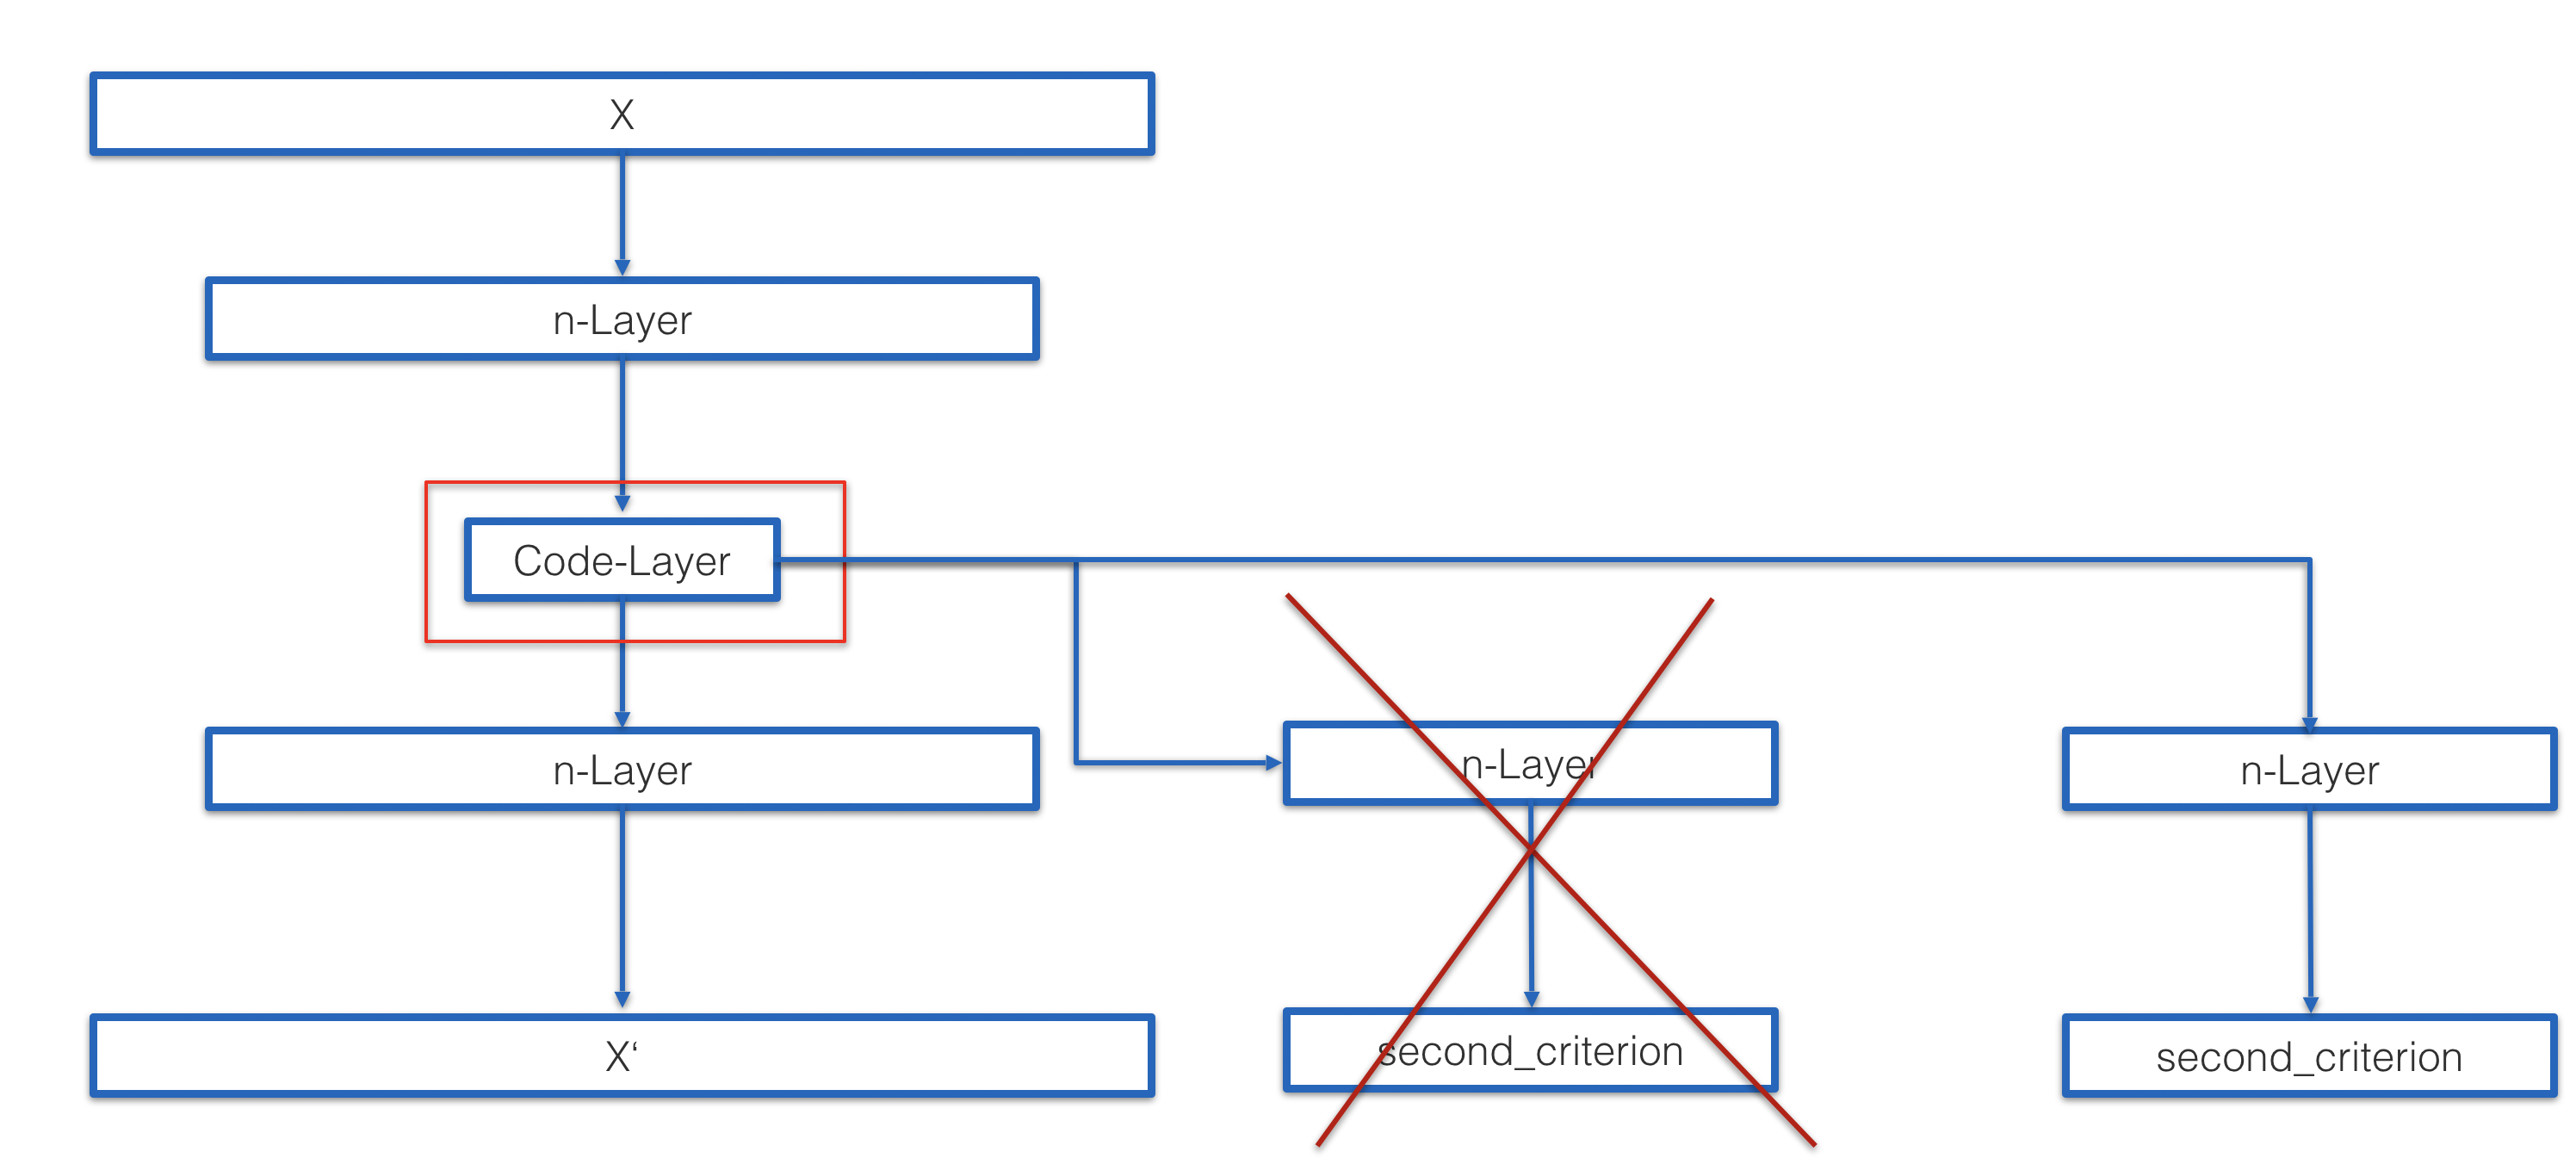
\includegraphics[width=0.5\textwidth, center]{bilder/Schema_Autoencoders/Schema_TSCAE.png}
		\caption[Schema TransferSecondCriterionAutoenocder]{Schema TransferSecondCriterionAutoenocder}
		\label{img:SchemaTSCAE}
	\end{figure}  

	
	\begin{figure}[h]
		\centering
		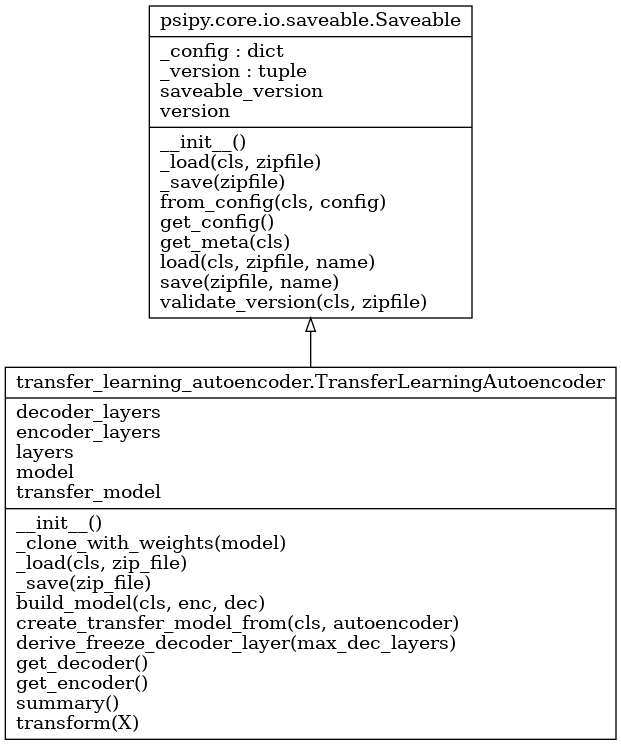
\includegraphics[width=0.5\textwidth, center]{bilder/Klassendiagramme/Klassendiagramm_TLCSCAE.png}
		\caption[Klassendiagramm TransferSecondCriterionAutoenocder]{Klassendiagramm TransferSecondCriterionAutoenocder}
		\label{img:KlassendiagrammTransferSecondCriterionAutoenocder}
	\end{figure}  
			
	\section{AutoTransferSecondCriterionAutoenocder}
	\label{sec:AutoTransferSecondCriterionAutoenocder}


	\begin{figure}[h]
		\centering
		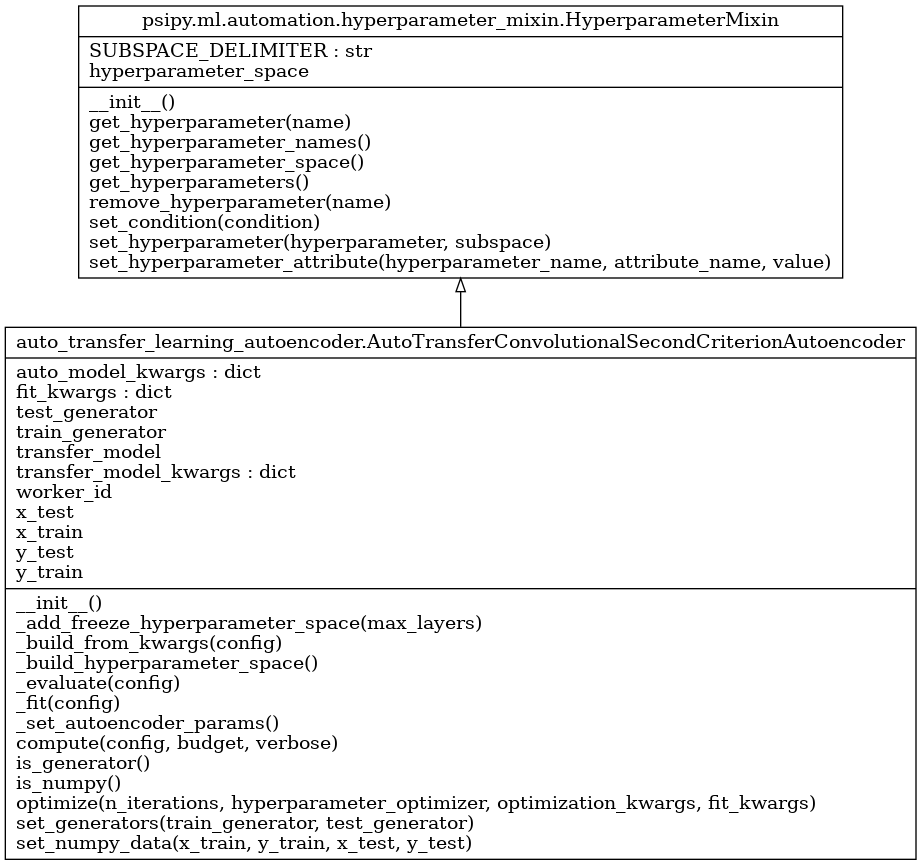
\includegraphics[width=0.5\textwidth, center]{bilder/Klassendiagramme/Klassendiagramm_AutoTLCSCAE.png}
		\caption[Klassendiagramm AutoTransferSecondCriterionAutoenocder]{Klassendiagramm AutoTransferSecondCriterionAutoenocder}
		\label{img:KlassendiagrammAutoTransferSecondCriterionAutoenocder}
	\end{figure}  